\documentclass{standalone}
\usepackage{tikz}
\usetikzlibrary{positioning,arrows.meta}

\begin{document}
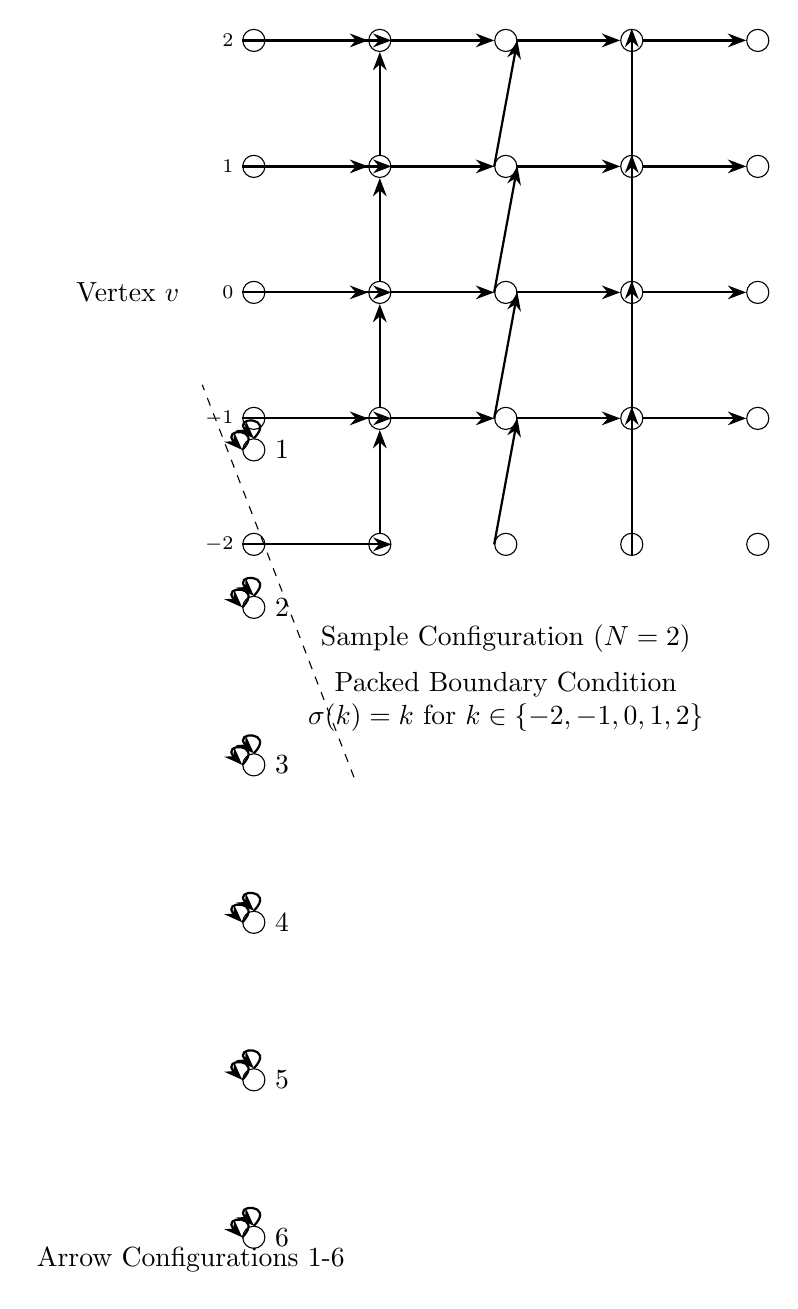
\begin{tikzpicture}[
    vertex/.style={circle, draw, minimum size=8pt, inner sep=0pt},
    arrow/.style={->, >=Stealth, thick},
    colorlabel/.style={font=\scriptsize, inner sep=1pt},
    scale=0.8
]

% Left panel: Arrow configuration labels
\begin{scope}[local bounding box=left]
    \node at (0,0) {Vertex $v$};
    \foreach \config [count=\i] in {
        {in=180,out=0,in=90,out=270},
        {in=180,out=0,in=270,out=90},
        {in=90,out=270,in=180,out=0},
        {in=90,out=270,in=0,out=180},
        {in=0,out=180,in=270,out=90},
        {in=0,out=180,in=90,out=270}
    }{
        \node[vertex] (v\i) at (2, -2.5*\i) {};
        \draw[arrow] (v\i.180) to[loop] (v\i.0);
        \draw[arrow] (v\i.90) to[loop] (v\i.270);
        \node[anchor=west] at (v\i.east) {\i};
    }
    \node[anchor=north] at (1,-15) {Arrow Configurations 1-6};
\end{scope}

% Right panel: Colored stochastic six-vertex model
\begin{scope}[local bounding box=right, xshift=6cm]
    % Grid setup
    \foreach \x in {-2,-1,0,1,2} {
        \foreach \y in {-2,-1,0,1,2} {
            \node[vertex] (n\x\y) at (\x*2, \y*2) {};
        }
    }

    % Left boundary arrows with colors
    \foreach \y [count=\i from -2] in {-2,-1,0,1,2} {
        \draw[arrow] (n-2\y.180) -- (n-1\y.0);
        \node[colorlabel,left=2pt] at (n-2\y.west) {$\y$};
    }

    % Internal arrows (sample configuration)
    \draw[arrow] (n-1-2.90) -- (n-1-1.270);
    \draw[arrow] (n-1-1.90) -- (n-10.270);
    \draw[arrow] (n-10.90) -- (n-11.270);
    \draw[arrow] (n-11.90) -- (n-12.270);
    
    \draw[arrow] (n0-2.180) -- (n0-1.0);
    \draw[arrow] (n0-1.180) -- (n00.0);
    \draw[arrow] (n00.180) -- (n01.0);
    \draw[arrow] (n01.180) -- (n02.0);
    
    \draw[arrow] (n1-2.270) -- (n1-1.90);
    \draw[arrow] (n1-1.270) -- (n10.90);
    \draw[arrow] (n10.270) -- (n11.90);
    \draw[arrow] (n11.270) -- (n12.90);
    
    \draw[arrow] (n-2-1.0) -- (n-1-1.180);
    \draw[arrow] (n-1-1.0) -- (n0-1.180);
    \draw[arrow] (n0-1.0) -- (n1-1.180);
    \draw[arrow] (n1-1.0) -- (n2-1.180);
    
    \draw[arrow] (n-20.0) -- (n-10.180);
    \draw[arrow] (n-10.0) -- (n00.180);
    \draw[arrow] (n00.0) -- (n10.180);
    \draw[arrow] (n10.0) -- (n20.180);
    
    \draw[arrow] (n-21.0) -- (n-11.180);
    \draw[arrow] (n-11.0) -- (n01.180);
    \draw[arrow] (n01.0) -- (n11.180);
    \draw[arrow] (n11.0) -- (n21.180);
    
    \draw[arrow] (n-22.0) -- (n-12.180);
    \draw[arrow] (n-12.0) -- (n02.180);
    \draw[arrow] (n02.0) -- (n12.180);
    \draw[arrow] (n12.0) -- (n22.180);

    % Annotations
    \node at (0, -5.5) {Sample Configuration ($N=2$)};
    \node[align=center] at (0, -6.5) {Packed Boundary Condition\\$\sigma(k)=k$ for $k\in\{-2,-1,0,1,2\}$};
\end{scope}

% Divider line
\draw[dashed] (left.east) -- (right.west);
\end{tikzpicture}
\end{document}